Time-series data refer as observation that collects over different period of time, Due to collection of data sampled during period of time there is chance of correlation between those observations. Time-series forecasting use past data to predict the future values. Time-series graph helps to identify the following characteristics

\begin{enumerate}
\item Seasonality
\item Trends
\item levels
\item Residual
\end{enumerate}
In time series data seasonality is a pattern of observations that occurs after particular time on repeated manner. it could be weekly, monthly, yearly or hourly bases. Trends existing when there is a constant linear upward or downward behaviour in the observation over period of time. For time-series analysis data should be stationary.

\textbf{What is Stationary in Time-Series model?}

In time-series stationary is the process in which mean, autocorrelation and standard variation of observation constant over the period of time. There is assumption about time-series that a time-series data is stationary. Stationary time-series data produce meaningful prediction of data. Consider the example of rainfall data which is different over the year, but the average of rainfall equal to small amount of year almost identical which produce the plausible result. There might be chances that for long period of time average of rainfall is not feasible i.e. increase in climate change. Indeed, statistical analysis of time-series  under the typical assumption of stationary of  observations. In real world some time-series dataset is not stationary hence adjustment or elimination of the trends and seasonality  must be required. The common approach to deal with non-stationary data to apply the difference of time-series data /cite{rao2008course}.   
 
\section{Classic Time Series Model}
\subsection{ ARIMA model}
In the time-series analysis white noise is the process where variation and mean of the observation are not constant or set to zero, hence the correlation between its observation is different. Since data is uncorrelated, previous observation is not useful to predict future data. Moving Average and Auto Regression is the model that helps to eliminate these violations in time series.
ARIMA  is the combination of Auto Regression (AR) with Moving Average (MA) with Integrated (I) module.
\begin{itemize}
\item AR:  Autoregressive is a model that current value considers as Xt calculated with a combination of past information n  values, Xt-1, Xt-2 Xt-n with white noise  (random error) Wt.

\(Xt = \Phi_{1}Xt-1 + \Phi_{2}Xt-2 + \Phi_{3}Xt-3 \Phi_{n}Xt-n  + Wt                                          \) 	
\item MA: AR model only uses past information of n values like  Xt-1, Xt-2, … Xt-n to forecast the future value with the current value of error Wt. AR model not used correlated error value of the past observations. Moving Average model is predicting the future data based on the previous value of error. Consider if you want to predict the Xt calculated by a combination of past ‘n’ values of errors,  Wt, Wt-1, Wt-2, … Wt-n.

\(Xt = \Phi_{1}Wt-1 + \Phi_{2}Wt-2 + \Phi_{3}Wt-3 …… \Phi_{n}Wt-n  + Wt 	\)
\item I: Integrated is a process when is useful when data is not stationary. If data is not stationary then the difference of each observation is calculated with the previous observation of timestamp and produces stationary time series data.                                     
\end{itemize}
 	
Each of these parameters set in the model, a standardized notation represent as  ARIMA (p,d,q) where each parameter substitute with different integer values.
\begin{itemize}
\item p: p denoted as lag order in Autoregressive that helps to select several past values to refer for predicting future data.
\item d: d is denoted as a difference that helps to use when data is not stationary. If data is not stationary after applying difference, then increase the degree of difference to stationary the time series data.
\item q:  q is denoted as a window size which normally provides a total number of lagged error of window size for forecasting.
\end{itemize}

\subsection{Vector Auto Regression (VAR)}
Vector Auto Regression is one of the prominent models in multivariate time-series data in which extension of the single univariate AR model to multivariate time-series AR model.
In the VAR model, each observation of the time series data not only depends on own its lag but also depends on the past observation of the data. A simple expression of the VAR model is given below

\(Xt =\Phi+ \Phi_{1}Xt-1 + \Phi_{2}Xt-2 + \Phi_{3}Xt-3 \Phi_{n}Xt-n  + Wt\)


\begin{figure}
  \centering
    
      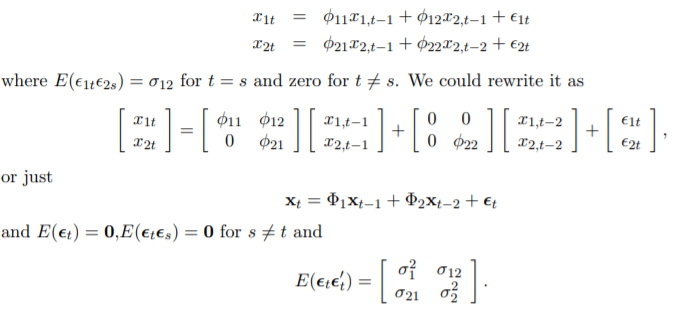
\includegraphics[width=1\textwidth]{VAR.png}
  \caption{Example of VAR model}
\end{figure}

 
\section{ Neural Network model}
Artificial Neural Network (ANN) is the mimic of a design of the human brain system. Similar like brain neurons an ANN use different layers of neurons which are connected perform complex computation task. The main difference between a single feed-forward network and RNN is there is one layer which is known as the recurrent layer that helps to store information about past information.  Figure \ref{fig:rnn} describes the recurrent network cell that helps to store long-term dependency of the input sequence in their recurrent layers. RNN is not useful while handling long-term dependency. Vanishing gradient or exploding the gradient such kind of phenomena encountered due to long-term dependency.

\begin{figure}
  \centering
    
      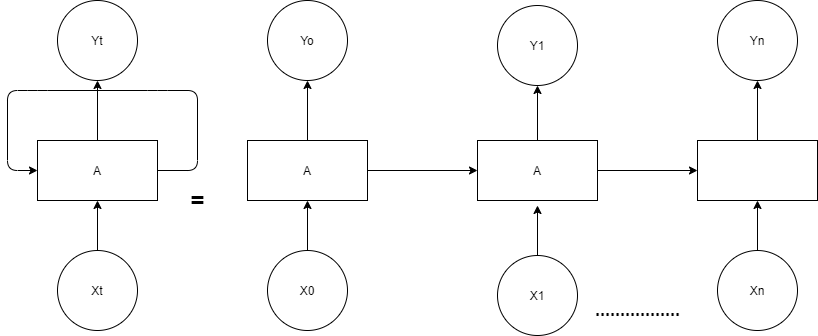
\includegraphics[width=1\textwidth]{RNN.png}
  \caption{Recurrent Neural cell}
  \label{fig:rnn}
\end{figure}

RNN performs backpropagation through time to adjust the weight and value of the hidden layers to minimize the loss function between true labels and predicted values. It improves the model using gradient descent which uses a learning rate to improve the model, if a learning rate is too low then multiplication and the complex calculation that is performed during each layer, hence vanishing gradient situation occurred after a long period. If the learning rate is too high then it misses global minima and exploding gradient after a long period. LSTM model solves the vanishing gradient problem \cite{lechner2020learning}.



\newpage{} 
\subsection{Long-Short Term Memory Model}
LSTM model solves the problem of vanishing gradient. LSTM handles short-term and long-term dependency simply and effectively with the help of gates which are as follows 
\begin{enumerate}
\item Forget gate: output of the previous timestamp pass to the current neuron of the observations it passes ht-1 and Xt to activation function which generate the value between 0 to 1. 0 represent as to forget the information while 1 represents as use the information.
\item Input gate: The input gate perform two operations which the main task to store the information in the cell. In the first task, information pass through the sigmoid function which updates the data based on the need. The second task is to convert information into the vector using the tanh activation function and combine both tasks into a new state.
\item Output gate: Output gate use two activation function on ht-1 and Xt with the combination of the result of activation function output gate information update the state of the information and using a combination of all gate state information, it passes to next neuron of the recurrent layer.
\end{enumerate} 
\begin{align*}
&\text{LSTM} : h^{l-1}_t, h^l_{t-1}, c^l_{t - 1} \rightarrow h^l_t, c^l_t\\
&\begin{pmatrix}i\\f\\o\\g\end{pmatrix} =
  \begin{pmatrix}\mathrm{sigm}\\\mathrm{sigm}\\\mathrm{sigm}\\\tanh\end{pmatrix}
  T_{2n,4n}\begin{pmatrix}h^{l - 1}_t\\h^l_{t-1}\end{pmatrix}\\
&c^l_t = f \odot c^l_{t-1} + i \odot g\\
&h^l_t = o \odot \tanh(c^l_t)\\
\end{align*}
In above equations,both activation function $\mathrm{sigm}$ and $\tanh$ are applied
gate wise. Figure \ref{fig:lstm} demonstrate the LSTM
equations.
\begin{figure}
  
      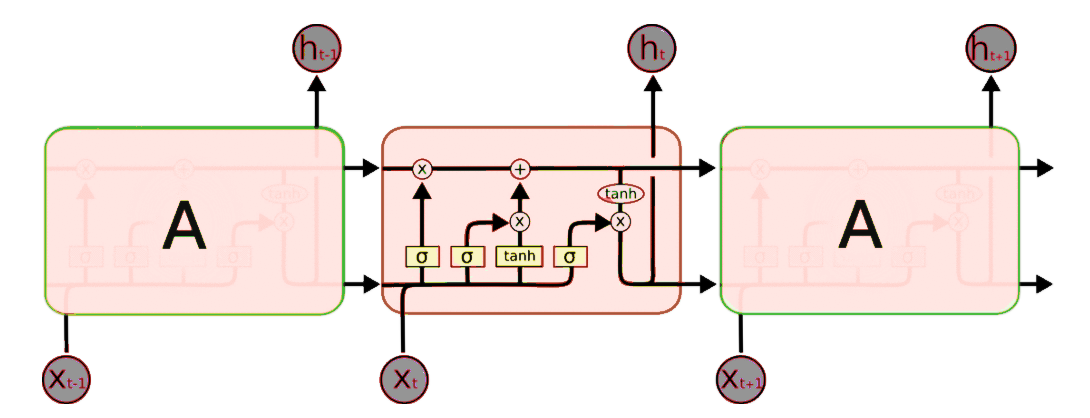
\includegraphics[width=1\textwidth]{LSTM.png}
  \caption{Long-Short Term Memory architecture}
  \label{fig:lstm}
\end{figure}

\subsection{ Bi-Directional LSTM}
A major drawback of  time-series data is model difficulty to store long-term dependency of the sequence model which result in a local minimum of the loss function during training a model goes into the negative direction of the gradient and while performing back-propagation  
It will multiply and iteratively become small after each operation which vanishing the gradient. As mentioned above LSTM use to solve the long-term dependency using complex architecture \cite{sundermeyer2012lstm}. LSTM only uses past information to predict the future data, while Bi-LSTM has two layers of LSTM which not only use past data but also use future data. It uses both forward and backward dependency to predict the outcome, both dependencies capture varying time-series data. The following diagram shows the full architecture of the Bi-LSTM in which two LSTM one in forwarding direction from 1 …T and second is in the backward direction from T … 1.
\begin{enumerate}
\item \(S_{ft}=f(A^{ft} X_{t} + D^{f} S_{ft-1} + B^{f} )\)
\item \(S_{bt}=f(A^{bt} X_{t} + D^{b} S_{bt-1} + B^{b} )\)
\item \(Y_{ft}=g(V^{f} S_{ft}+V^{b} S_{bt}+B ^{0})\)
\end{enumerate}
the above equation two layers $S_{ft}$ and $S_{bt}$ of LSTM both are running in opposite direction $A^{bt}$ and $D^{b}$ are the weight of backward while $A^{ft}$ and $D^{f}$ are the weight metrics of the forward LSTM network. $V^{f}$ and $V^{b}$ are known as output of both layers.
\begin{figure}
      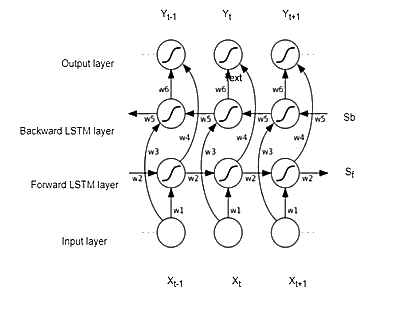
\includegraphics[width=1\textwidth]{Bilstm.png}
  \caption{Bi-directional Long-Short Term Memory architecture}
  \label{fig:bilstm}
\end{figure}

